\documentclass{astroedu-lab}

\begin{document}

\pagestyle{plain}

\begin{problem}{\huge Лабораторная работа 1.3.2\\\\Определение модуля кручения\\\\Выполнил Жданов Елисей Б01-205}

\section{Цель работы:}

Определение модулей кручения и сдвига для проволоки по измерениям периодов крутильных колебаний подвешенного на ней маятника.

\section{Оборудование:}

Проволока из исследуемого материала, грузы, секундомер, микрометр, рулетка, линейка.

\section{Теория деформации кручения:}

Когда мы закручиваем стержни круглого сечения, распределение деформаций и напряжений одинаково по длине стержня только вдали от мест, где прикладыпаются закручивающиие моменты. Для этих областей можно считать, что каждое поперечное сечение поворачивается как жесткое, то есть частички материала не сходят с тех радиальных линий, на которых они находились вначале, и все эти радиальные линии поворачиваются на один и тот же угол. Напряженное состояние, которое при этом возникает, называется чистым кручением. Далее будет показано, что касательные напряжения в поперечном сечении увеличиваются пропорционально расстоянию от оси вращения.

\newpage

\begin{wrapfigure}{r}{0.6\textwidth}
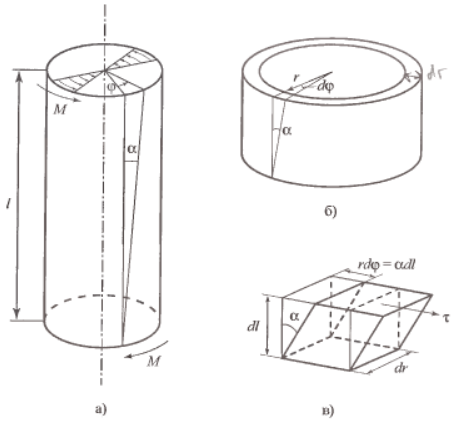
\includegraphics[width=0.6\textwidth]{theory_1.png}
\caption{}
\label{ris:image}
\end{wrapfigure}.

Посмотрим на часть закручиваемого круглого цилиндра, имеющую длину $l$, которая изображена на рис. 1а. Любая прямая линия, проведенная до закручивания цилиндра по частицам материала и параллельная оси симметрии, при закручивании превращается в спираль (винтовую линию). Сечения, находящиеся на расстоянии $l$, повернуты на угол $\varphi$.

Начнем с рассмотрения в цилиндре колечка произвольного радиуса $r$ с бесконечно малой толщиной $d r$ и бесконечно малой высотой $d l$, показянное на рис.1б. При закручивании верхнее сечение колечка поворачиваегся относительно нижнего на угол $d \varphi$, а образующая цилиндрнческой поверхности колечка $d l$ наклоняется на утол $\alpha$, преДставляя элемент тех $\alpha$ можно написать
$$
\alpha d l=r d s .
$$
Видно, что $\alpha$ возрастет с увеличением расстояншя от оси цилиндра $r$. На рис. 1в показан элемент колечка, в котором происходит сдвиговая деформация. Касательное напряжение $\tau$ связано с углом сдвига $\alpha$ линейной зависимостью, в которую входит модуль сдвига G

\begin{equation}
	\tau = G \alpha
\end{equation}

Касательно напряжение $\tau$ пропорционально $\alpha$ и, следовательно, тоже растет с увеличением расстояния от оси цилиндра, о чем уже говорилось выше. Как результат, получим

\begin{equation}
	\tau = G r \frac{d \varphi}{d l}
\end{equation}

Эти касательные напряжения создают момент сил относительно оси цилиндра

\begin{equation}
	d M = 2 \pi r d r \cdot \tau \cdot r
\end{equation}

Суммарный момент сил, действующий на всем поперечном сечении цилиндра, находится интегрированием от оси цилиндра до радиуса R

\begin{equation}
	M = 2 \pi G \frac{d \varphi}{d l} \int\limits_0^R r^3 d r = \pi G \frac{d \varphi}{d l} \cdot \frac{R^4}{2}
\end{equation}

Этот момент не меняется по длине цилиндра. Переменные под дифференциалами независимы, а значит можно записать итоговую формулу

\begin{equation}
	M = 2 \pi G \frac{d \varphi}{d l} \int\limits_0^R r^3 d r = \pi G \frac{\varphi}{l} \cdot \frac{R^4}{2} = f \varphi
\end{equation}

Модулем кручения f обозначено следующее соотношение

\begin{equation}
	f = \frac{\pi R^4 G}{2 l}
\end{equation}

Разумеется, зависимость работает только при небольших сдвигах.

\section{Описание установки:}

\begin{wrapfigure}{r}{0.6\textwidth}
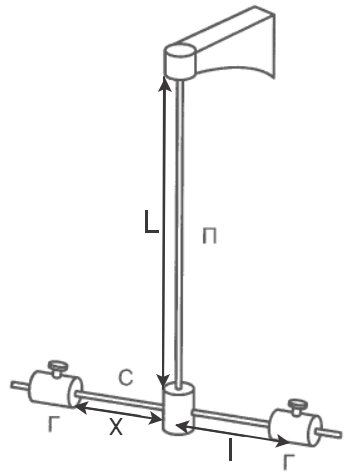
\includegraphics[width=0.6\textwidth]{state_1.png}
\caption{}
\label{ris:image}
\end{wrapfigure}.

Экспериментальная установка, используемая в этой части работы,
изображена, на рис. 3 и состоит из длинной вертикально висящей проволоки П, к нижнему концу которой прикреплен горизонтальный металлический стержень С с двумя симметрично расположенными грузами
Г. Их положение на стержне можно фиксировать. Верхний конец проволоки зажат в пангу и при помощи специального приспособления может
вместе с цангой поворачиваться вокруг вертикальной оси. Таким способом в системе можно возбуждать крутильные колебания. Вралцение стержня С с закрепленными на нем грузами Г вокруг вертикальной оси происходит под действием упругого момента, возникающего в проволоке. Это вращение описывается уравнением

\begin{equation}
	M = I \frac{d^2 \varphi}{d t^2}
\end{equation}

Выражу момент инерции системы через её составляющие

\begin{equation}
	I = I_0 + 2 m l^2
\end{equation}

Согласно рисунку буду вычислять l используя линейные размеры грузов и расстояние x, замеряемое штангенциркулем. Далее подробнее.

Согласно теории кручения

\begin{equation}
	\omega^2 = \frac{f}{I}
\end{equation}

Подставляем в уравнение колебаний

\begin{equation}
	\frac{d^2 \varphi}{d t^2} + \omega^2 \varphi = 0
\end{equation}

Решение дифференциального уравнения

\begin{equation}
	\varphi = \varphi_0 \sin{\left(\omega t + \theta\right)}
\end{equation}

Период же равен

\begin{equation}
	T = 2 \pi \sqrt{\frac{I}{f}}
\end{equation}

Важно учеть затухание и грамотно им пренебречь.

\section{Измерения и обработка:}

0) Приведу замеры размеров, которые будут использоваться в дальнейшем

Взвешу груз на электронных весах

\begin{equation}
	m = 375.6 \text{ г}
\end{equation}

Длина проволки $L = 1.766 \pm 0.001$ м; её радиус $R = 1.99 \pm 0.01$ мм.



1) Установлю амплитуду в $30^\circ$ и $15^\circ$.

Периоды 10 колебаний составляют соответственно 34.05 и 34.01 сек, что действительно близко. Затуханием можно спокойно пренебречь.

2) Уменьшение амплитуды составляет $2^\circ $ (от $30^\circ$ до $28^\circ$). Это тоже очень малое затухание, которым можно пренебречь()тем более меньшее половины исходной амплитуды).

3) Приведу таблицу замеров ниже

\begin{center}
\begin{tabular}[t]{|c|l|l|}
\hline
10x T, сек & \multicolumn{2}{|c|}{$x_i$, см} \\
\hline
34.01 & 6.87 & 6.83\\
31.26 & 5.81 & 5.77\\
28.77 & 4.84 & 4.79\\
26.23 & 3.83 & 3.81\\
23.85 & 2.84 & 2.83\\

\hline
\end{tabular}
\end{center}


Таблица с необходимыми пересчетами

\begin{center}
\begin{tabular}[t]{|c|l|l|l|l|}
\hline
T, сек & x, см & l, см & $T^2$, сек & $l^2$, см$^2$\\
\hline
3.401  & 6.85  & 11.35 & $(11.57 \pm 0.003)$ 	 & $(128.8 \pm 0.2)$ \\
3.126  & 5.79  & 10.29 & $(9.77 \pm  0.003)$	 & $(105.9 \pm 0.2)$ \\
2.877  & 4.82  & 9.32  & $(8.28 \pm  0.003)$	 & $(86.9 \pm 0.2)$ \\
2.623  & 3.82  & 8.32  & $(6.88 \pm  0.003)$	 & $(69.2 \pm 0.2)$ \\
2.385  & 2.84  & 7.34  & $(5.69 \pm  0.002)$	 & $(53.9 \pm 0.1)$ \\

\hline
\end{tabular}
\end{center}

Погрешностью периода буду в дальнешем пренебрегать, поскольку она на порядок ниже погрешности длины.

Получу подстановкой момента инерции системы в формулу для периода зависимость, график которой я буду строить

\begin{equation}
	T^2 = 4 \pi^2 \frac{I_0}{f} + \frac{8 \pi^2 m}{f} \cdot l^2
\end{equation}

Зависимость вида y = ax + b, строю график $T^2$ от $l^2$

\begin{center}
\begin{tikzpicture}
\begin{axis}[
	width=250,
	xlabel     = \text{$l^2$ [см]$^2$}, % label x axis
    ylabel     = \text{$T^2$ [сек]$^2$}, % label y axis
	]
\addplot[mark = *] table {
	x     y
128.8 11.57
105.9 9.77
86.9 8.28
69.2 6.88
53.9 5.69
128.8 11.57
};
\end{axis}
\end{tikzpicture}
\end{center}

Корелляция идеальная, кресты погрешностей не удовлетворяют масштабу графика

Итоговый коэффициент наклона(в СИ)

\begin{equation}
	k = (785 \pm 3) \frac{\text{сек}^2}{\text{м}^2}
\end{equation}

4) Модуль кручения

\begin{equation}
	f = \frac{8 \pi^2 m}{k} = (0.0378 \pm 0.0001) \text{ [СИ]}
\end{equation}

И наконец, модуль сдвига

\begin{equation}
	G = \frac{2 l f}{\pi R^4} = (43 \pm 1) \text{ ГПа}
\end{equation}

Погрешность G(на f влияет только погрешность k)

\begin{equation}
	\varepsilon_G = 4 \varepsilon_R +\varepsilon_f
\end{equation}

\section{Время делать выводы:}

В соответствии с справочными данными, полученный модуль сдвига весьма похож на значение у меди(46.5 ГПа). Вероятно, проволка медная, более того, образец для замера диаметра был кристально-медного цвета. Отличие менее, чем на 10$\%$ от табличных данных считаю весьма достоиным результатом, говорящем скорее о типе того или иного используемого сплава.

Вспоминая о цели работы, можно заметить, что она выполнена, то есть найдены модули сдвига и кручения данной проволки.

\end{problem}
\end{document}